%% Section that includes the experiments performed.

This section describes the accomplished experiments that prove how the developed system fulfills SKA's requirements for the PPS distribution system. The first experiment is a general characterization of the developed platform. The second one, tests the equipment in a realistic network topology to evaluate the performance in a possible deployment. The last experiments evaluates the influence of some typical events, such as traffic, temperature fluctuation or \textcolor{blue}{something else} in a network deployment using the WR-ZEN.

Performance of the new WR platform is measured using multiple equipment, and obtained results have been compared to WRS's performance because of it's electronic design is considered as \ftglnote{en serio?}reference for WR technology. The list of the equipment and materials used for the experiments is the following:

\begin{itemize}
    \item Three White Rabbit Switches to simulate a typical WR network. All of them have hardware version 3.4 and 5.0 of firmware.
    \item A White Rabbit ZEN Time Provider (WR-ZEN TP) to test the performance of the new developed platform as node of a WR network. The firmware version is 1.2.
    \item Phase noise plots, ADEV, TDEV and TIE measures have been taken using a Symmetricom 3120A.
    \item The 3120A needs an external stable clock reference. That reference is also needed as input for the WR equipment when Grand Master mode is set. \ftglnote{Creo que sería necesario comentar aquí que hemos diseñado una placa para poder sacar la referencia de 10Mhz doble y un PPS, pero como lo ha hecho 7s no se como ponerlo...}A Morion MV89 Oven Controlled Crystal Oscillator (OCXO) has been used as clock reference for the experiments.
    \item Multiple components for the setup of the equipment:
    \begin{itemize}
        \item Small form-factor pluggable transceptors (SFPs) to stablish the link between WR devices.  \textcolor{blue}{\textit{TODO:} Completar cuando se hayan usado}
        \item Optical fiber links. \textcolor{blue}{\textit{TODO:} Completar con las fibras que se hayan usado}
        \item \textcolor{blue}{\textit{TODO:} Something else?}
    \end{itemize}
    \item \textcolor{blue}{\textit{TODO:} Completar conforme se hagan medidas}
\end{itemize}

\subsection{Characterization of the WR-ZEN platform}
\label{subsec: charact_zen}

% Aquí las pruebas típicas de caracterización

The new components included in the clocking's scheme of the WR-ZEN, described in section \ftglnote{Meter ref cuando esté integrado en el resto} 4.1, offer a performance improvement respect to previous WR designs, such as the WRS. 

\missingfigure{Esquema de las medidas realizadas}

The following experiments evaluate phase noise performance of the frequency transfer in WR at different scenarios: a) Grand Master mode, to evaluate how the WR-ZEN syntonizes to an external reference clock. b) Master mode, that reflects the characteristics of the new internal XO of the WR-ZEN. c) Slave mode, to see the behavior of the new design as slave node of the network.

The Free running mode (FR) is not affected by the WR's logic, it is mostly influenced by noise of the crystal oscillator (XO). \textcolor{blue}{TODO: Completar haciendo referencia a la sección de hardware.}

\ftgnote{Las figuras de Phase Noise juntas se ven regular, pero separadas parece que estamos tirando espacio para rellenar...}
\begin{figure}
    \centering
    \begin{subfigure}[t]{0.45\textwidth}
        \includegraphics[width=\textwidth]{../measures/img/zen_all}
        \caption[Phase noise plot of the WR-ZEN]{The figure shows the Phase noise plot for the WR-ZEN in the Grand Master, Free Running and Slave modes. Sine wave output is compared to CMOS output.}
        \label{fig:zen_pn_all}
    \end{subfigure}
    ~ % This symbol adds a white space between images
    \begin{subfigure}[t]{0.45\textwidth}
         \includegraphics[width=\textwidth]{../measures/img/zen_vs_wrs}
         \caption[Phase noise plot of the WR-ZEN vs WRS]{The figure includes the same phase noise measures for the WRS. In this plot, only the CMOS outputs appear because the WRS doesn't have sine wave output signals.}
         \label{fig:zen_vs_wrs}
    \end{subfigure}
\end{figure}

The following experiments evaluate phase noise performance of the frequency transfer in WR at different scenarios: a) Grand Master mode, to evaluate how the WR-ZEN syntonizes to an external reference clock. b) Master mode, that reflects the characteristics of the new internal XO of the WR-ZEN. c) Slave mode, to see the behavior of the new design as slave node of the network. Different configurations are depicted in fig. ?? to allow the reproduction of the different experiments of this paper.

The Free running mode (FR) is not affected by the WR's logic, it is mostly influenced by noise of the crystal oscillator (XO). A master node is placed at top of a timing network hierarchy, and unlike a Grand Master node, it is not locked to any external reference. So that, a master node with an improved stability will benefit the performance of all the downlink devices connected to it.

It is also relevant to test the performance of the system when locking to an external reference in Grand master mode. Additive noise of the WR-ZEN will be propagated downstream, decreasing the quality of the Grand master's reference clock. It's very important that the system adds low noise in order to not degrade the quality of the external reference clock.

Results included in table \ref{tab:pn_results} ... \textcolor{blue}{TODO: hablar de la frecuencia de corte del softpll y del ddmtd.}
    
\begin{table*}\centering
     \ra{0.8}
     \begin{tabular}{@{} rcccc@{}}%\toprule
         & \multicolumn{4}{c}{\bfseries{RMS jitter (ps)}} \\
         \cmidrule(l){2-5}
         & 1Hz-10Hz & 10Hz-1kHz & 1kHz-100kHz  & 1Hz-100kHz \\ \midrule
         \textbf{Free running}\\
         \small{WRS (CMOS)}             & 62  & 1.7  & 1.1  & 62  \\
         \small{WR-ZEN (\textit{sine})} & 2.1 & 0.24 & 1.4  & 2.5 \\
         \small{WR-ZEN (\textit{CMOS})} & 1.9 & 0.21 & 0.26 & 1.9 \\
         \cmidrule(l){2-5}
         
         \textbf{Grand Master}\\
         \small{WRS (CMOS)}             & 7.3 & 6.7 & 1.1 & 9.9\\
         \small{WR-ZEN (\textit{CMOS})} & 2.8 & 6.2 & 0.26 & 6.8\\
         \cmidrule(l){2-5}
         
         \textbf{Slave node}\\
         \small{WRS (CMOS)}             & 4.9 & 8.2 & 1.2  & 9.7\\
         \small{WR-ZEN (\textit{CMOS})} & 8.5 & 9.3 & 0.24 & 13\\
         
         \bottomrule
        \end{tabular}
        \caption{Phase Noise results extracted from plots in figure \ref{fig:zen_pn_all} and \ref{fig:zen_vs_wrs}.}
        \label{tab:pn_results}
\end{table*}

The slave mode results show that WR-ZEN performs slightly worse than WRS. Noise between 1 Hz and 20 Hz increases the RMS Jitter of the WR-ZEN. \textcolor{blue}{This may be caused by a poor adjustment of the PI control.}

\missingfigure{Allan deviation plot}

\subsection{Network experiment} %% Buscar un nombre mejor
\label{subsec: net_exp}

The next experiment covers the analysis of timing distribution over a WR network formed by a WRS in the top of the hierarchy locked to an external reference (Grand Master), an intermediate WRS and a final node, the WR-ZEN. We planned to reproduce an example of time distribution for the SKA facilities where it won't be there so many hops between the clock reference and end nodes. For the experiment we kept devices under laboratory conditions: temperature and humidity controlled, absence of external noise sources and so on. For a more realistic tests under changing conditions, see Paul Boven's results in \cite{paultests}. He performed some measures using two WR-ZEN connected by tens of kilometers fiber links in controlled conditions (climate chamber) and with a real fiber deploy in South Africa.\ftglnote{Completar}

\begin{figure}[H]
    \begin{subfigure}[t]{.35\textwidth}
        \centering
        \includegraphics[width=\textwidth]{img/prueba1_pps.png}
        \caption{Setup for the PPS results of the WR-ZEN directly connected to the Grand Master WRS.}
        \label{fig:prueba1_sch}
    \end{subfigure}
    ~
    \begin{subfigure}[t]{.60\textwidth}
        \centering
        \includegraphics[width=\textwidth]{img/prueba2-3_pps.png}
        \caption{Setup for the network experiment taking measures from WRS L2 and the end node WR-ZEN.}
        \label{fig:prueba2_sch}
    \end{subfigure}
\end{figure}

Some long-term stability results are presented in table \ref{tab:netres} and fig. \ref{fig:tdev_plots} because of the importance of that kind of measures for time distribution networks. This time, we have take the PPS outputs from WRS and WR-ZEN and we have performed some long time measurements and plotted them with a Time Deviation (TDEV) analysis. \ftglnote{Meter la fórmula del TDEV($\tau$) concreto y sacar un par de valores}

Phase difference on each hop can be checked on figure ??.

\begin{figure}[H]
    \begin{subfigure}[t]{.45\textwidth}
        \centering
        \includegraphics[width=\textwidth]{img/pps_p1.png}
        \caption{TDEV for the first configuration.}
        \label{fig:pps_p1}
    \end{subfigure}
    ~
    \begin{subfigure}[t]{.45\textwidth}
        \centering
        \includegraphics[width=\textwidth]{img/pps_p2.png}
        \caption{TDEV for the second configuration.}
        \label{fig:pps_p2}
    \end{subfigure}
    
    \centering
    \begin{subfigure}[t]{.45\textwidth}
        \centering
        \includegraphics[width=\textwidth]{img/pps_p3.png}
        \caption{TDEV for the third configuration.}
        \label{fig:pps_p3}
    \end{subfigure}
    \caption{Time Deviation plots for the PPS distribution system}
    \label{fig:tdev_plots}
\end{figure}

\begin{table*}\centering
    \begin{tabular}{cccc}
        & 1st config. & 2nd config. & 3rd config \\ 
        Max & 118 ps & 353 ps & 646 ps \\ 
        Min & -27 ps & 196 ps & 524 ps \\ 
        Pk-to-Pk & 146 ps & 156 ps & 122 ps \\ 
        Mean & 50 ps & 273 ps & 15 ps \\ 
        $\sigma$ & 19 ps & 23 ps & 15 ps \\ 
    \end{tabular}
    \caption{Time results from network experiment.}
    \label{tab:netres}
\end{table*}

\ftgnote{TODO: format this table}

\begin{figure}[H]
    \begin{subfigure}[t]{.3\textwidth}
        \centering
        \includegraphics[width=\textwidth]{img/prueba1_pd.png}
        \caption{Phase difference for experiment 1}
        \label{fig:prueba1_pd}
    \end{subfigure}
    ~
    \begin{subfigure}[t]{.30\textwidth}
        \centering
        \includegraphics[width=\textwidth]{img/prueba2_pd.png}
        \caption{Phase Difference for experiment 2}
        \label{fig:prueba2_pd}
    \end{subfigure}
    ~
    \begin{subfigure}[t]{.3\textwidth}
        \centering
        \includegraphics[width=\textwidth]{img/prueba3_pd.png}
        \caption{Phase difference for experiment 3}
        \label{fig:prueba3_pd}
    \end{subfigure}
    \caption{Phase difference plots for the different configurations of the network PPS stability analysis.}
\end{figure}

\textit{TODO:} Hablar del tipo de ruido predominante en las gráficas de TDEV 
cuando las repita y se verifiquen. Reemplazar Pk-to-Pk por MTIE.


\subsection{Fiber operational temperature influence on time accuracy}

One of the key aspects of the timing solution for the SKA facilities is the 
influence evaluation of the external elements in the timing performance. 
Synchronization signals are spread over hundred of nodes which are connected by 
long distance fiber links. Meteorological elements, such as wind or large 
 temperature changes, can alter propagation delays over the fiber 
links. The timing solution must compensate appropriately those effects in order 
to maintain the synchronization performance inside the limits required by the 
SKA's infrastructure.

On this contribution we've focused on the temperature change effect on the 
\textit{round-trip} (RTT) time and the PPS's performance. To evaluate that, we 
own a 
climate chamber in the laboratory and some fiber spools of tens of kilometers. 
We couldn't evaluate properly wind impact with our equipment, because of this, 
the experiments will only determine temperature effect on synchronization.

\ftgnote{Aquí un párrafo mencionando los efectos físicos sobre los haces de luz 
que viajan por la fibra al cambiar la temperatura. Índice de refracción. 
Aportar referencias!!!!}

Theoretically, WR, is able to dynamically calibrate the master to slave 
propagation delay from the total \textit{round-trip} time, \ftglnote{se 
necesita una ref aquí?} and therefore PPS offset shall maintain constant even 
when the propagation delay changes. The accurate estimation of the one-way 
propagation delay is achieved by the use of a constant value, $\alpha$, which 
express the ratio between propagation times with the two wavelengths used in 
the WR link. A complete explanation of the link model could be read in 
\cite{Wlostowski2011} and \cite{Daniluk2012}.

In the real world, $\alpha$ is temperature dependent, because of the change in 
the refraction index due to a temperature variation in the fiber. For small and 
mid-distance links, in laboratory conditions, $\alpha$ is nearly negligible and 
the current link model works very well. The WR network in SKA will be formed by 
long distance links exposed to external elements. In the concrete situation of 
the South Africa facilities, the chosen location was the Karoo region. 
\ftglnote{comprobar eso porque lo he sacado de Wikipedia} This region is a 
semi-desert area, very adequate to reduce human interferences in the high 
resolution data acquisition equipment, but with a inconvenient respec to the 
temperature point of view: desertic zones have a high difference between day 
and night temperatures.

We performed a series of experiments introducing a 50 km length fiber spool in 
a climate chamber. The RTT and the PPS's offset between master and slave were 
evaluated for a temperature range from 20 ºC to 50 ºC with 10 ºC steps. The 
average temperature difference between day and night in the Karoo region on 
each month is below 20 ºC, so the experiment covers comfortably the expected 
temperature operation conditions.

Our work hypothesis is that PPS's offset should keep constant for a varying 
RTT, in other words, the offset and the RTT do not present any kind of 
relationship between them. To prove this hypothesis, we have simulated the 
expected temperature conditions for a 50km fiber link using a climate chamber. 
Outside, in laboratory conditions, two WR-ZENs are connected using that fiber 
in a master-slave configuration. Then we've measured the offset of the PPS 
signal from slave to master with a timer (Keysight 53230A). The usual SFPs in 
WR deployments were not suitable for this experiment due to the long distance 
fiber link. We've used bidir SFPs from FiberStore with support up to 80 km 
distance links using 1550/1490 nm wavelengths. The setup schema is depicted in 
Figure ??. \ftglnote{hacer figura}

We had to perform the WR calibration procedure described in \cite{man:calib} to 
properly compensate the characteristic delays of the WR-ZEN board and the 
$\alpha$ constant of the used wavelengths. Once all the equipment was setup and 
calibrated, we started the thermal characterization of the link. To do that, we 
accomplished 4 independent experiments, where each one was related to one of 
the operation temperatures for the fiber spool. We started the measurement when 
the temperature of the system reached a stable point according to the targets. 

\begin{table*}\centering
	\ra{0.8}
	\begin{tabular}{@{} cccccc@{}}%\toprule
		& \multicolumn{2}{c}{\bfseries{RTT (ps)}} & &
		\multicolumn{2}{c}{\bfseries{PPS $offset_{SM}$ (ps)}} \\
		\cmidrule(l){2-3}  \cmidrule{5-6}
		\textbf{Spool temp (ºC)} & $\overline{x}$ & $s$ & & $\overline{x}$ 
		& $s$ \\ \midrule
	\small{20} & 479347020 & 365 & & 194 & 17 \\
	\small{30} & 478503719 & 50  & & 203 & 17 \\
	\small{40} & 478533492 & 807 & & 150 & 17 \\
	\small{50} & 478567050 & 399 & & 110 & 14 \\
	\bottomrule
	\end{tabular}
	\caption{Results of the thermal characterization for an operational fiber 
		temperature in range 20ºC to 50ºC with 10ºC steps.}
	\label{tab:temp}
\end{table*}

The most relevant results are included in Table \ref{tab:temp}: (i) the mean 
value of RTT and PPS offset samples, and (ii) their sample standard deviation. 
A total of 7200 samples (2 hours) have been used to compute the presented 
statistics. Round-trip time average for all the samples is 479347020 ps ($s=365 
ps$), and for the PPS offset we have an average of 194 ps ($s=17 ps$)
The correlation coefficient, expressed by the formula \ref{eq:r}, of the 
variables Offset (O) and RTT (R) is 0.08. This indicates a very weak linear 
relationship between both variables, which is just what we expected with our 
hypothesis.
Figure \ref{fig:ppsvsrtt} joins all the data from the experiments with 
different fiber temperature and makes visual that both variables are weakly 
related. Red line represents a fit linear model for the PPS offset given a RTT 
value. Line's slope is positive but with a very low increment. The reason for 
the deviation from 0 could be the use of a computed approximation of the real 
$\alpha$ value. 

\begin{equation}\label{eq:r}
r_{OR} = \frac{s_{OR}}{s_{O} s_{R}}
\end{equation}

The expected slave to master PPS offset related to distance and temperature of 
the fiber link is defined by the expression \ref{eq:offset}. We experimentally 
obtained that $k=0.13 ps$ \ftglnote{a javi: este k lo calculo de los valores 
medios experimentales, eso está bien? sería mejor con los del peor de los 
casos?}
\ftgnote{Comprobar el modelo haciendo una prueba con una fibra de 20km!!!!}

\begin{equation}\label{eq:offset}
	\hat{offset_{SM}} (T,d) = \frac {k ps} {T ºC \cdot d km}
\end{equation}

\begin{figure}
	\centering
	\includegraphics[width=1\linewidth]{img/ppsvsrtt}
	\caption[Evolution of the PPS offset and the RTT on multiple working 
	temperature for the fiber link]{Evolution of the PPS offset and the RTT on 
	multiple working temperature for the fiber link}
	\label{fig:ppsvsrtt}
\end{figure}
